\documentclass[12pt]{article}
\usepackage{amsmath,epsfig,calc,capt-of,ifthen}

%%%%%%%%%% Start TeXmacs macros
\newcommand{\tmem}[1]{{\em #1\/}}
\newcommand{\tmfloatcontents}{}
\newlength{\tmfloatwidth}
\newcommand{\tmfloat}[5]{
  \renewcommand{\tmfloatcontents}{#4}
  \setlength{\tmfloatwidth}{\widthof{\tmfloatcontents}+1in}
  \ifthenelse{\equal{#2}{small}}
    {\ifthenelse{\lengthtest{\tmfloatwidth > \linewidth}}
      {\setlength{\tmfloatwidth}{\linewidth}}{}}
    {\setlength{\tmfloatwidth}{\linewidth}}  \begin{minipage}[#1]{\tmfloatwidth}
    \begin{center}
      \tmfloatcontents
      \captionof{#3}{#5}
    \end{center}
  \end{minipage}}
%%%%%%%%%% End TeXmacs macros

\begin{document}
\title{Best Reply Behavior}
\author{Michael Peters}
\date{\today}
\maketitle

\section{Introduction}
So far, we have concentrated on individual optimization. This unified way of
thinking about individual behavior makes it possible to understand a number of
interesting economic problems. Some of these will be discussed in coming
chapters. However, the biggest insights in economics come from thinking about
group behavior. Individual and group behavior are tied together in economics
by best reply behavior.

As you have seen in prior readings, the solutions to individual maximization
problems depend on characteristics of the environment. When many people make
maximizing decisions at the same time, their choices may or may not be
consistent with one another. Perhaps the biggest insight of all in economics
is that consistency restrictions on peoples' choices will impose restrictions
on the set of environments that we should ever expect to see.

The oldest application of this idea is the one that you probably saw in
operation in your first year economics course. Every consumer's demand for
every good depends on the price that she thinks prevails for that good. If
consumers' beliefs about these prices are completely arbitrary, then some
goods will be in excess demand and some in excess supply. As a consequence,
all consumers should have the same belief about the price at which they can
buy each good, and this belief should be that the price will be the one at
which aggregate demand and aggregate supply are equal. This is where the
concept of a market comes from. A market isn't a physical location where
traders buy and sell, rather it is a state of beliefs that result in a kind of
consistent and predictable behavior on the part of a large group of individual
decision makers.

Prior to John Nash and game theory, economics couldn't really get much beyond
markets in thinking about group behavior. In cases where markets obviously
couldn't give a good description of behavior, very special models were
proposed - for example, the monopoly model to deal with the obvious cases in
which firms are not price takers. Nash showed that you can use the consistency
of individual decisions in a much broader way to understand many non-market
problems as well.

The basic idea behind Nash equilibrium is that instead of forming beliefs
about prices, people form beliefs about what other people will do. Fixing
these beliefs leads us back directly to the maximization framework that we
have been studying so far. In order think about consistency among these
beliefs, we have to extend the kind of reasoning we have been using to derive
the demand curve to a much more flexible description of best reply behavior.

\section{Consumption Theory with Externalities}

To understand this method, lets modify our description of the individual
choice problem slightly. As before, lets suppose that there are two goods. The
price of good $y$ will be 1, and the price of good $x$ will be $p$ throughout
this argument. However, lets suppose that there are two consumers instead of
just 1. Each consumer has $W$ to spend on $x$ and $y$. The utility that each
person gets for good $x$ depends positively on the amount of good $x$ that the
{\tmem{other}} person chooses to consume. This is called a {\tmem{positive
consumption externality}}. Such externalities are everywhere. Movies and
novels are great examples - they are fine by themselves, but they are even
more enjoyable if your friends have seen the same movie or read the same book,
because then you can discuss it. On the margin you might be inclined to go to
see a certain movie just because you know one of your friends has already seen
it.

Lets call the consumers Alice and Bob, denoting Alice's consumption bundle by
$( x_a, y_a )$ and Bob's by $( x_b, y_b ) .$ Alice's utility function is $u (
x_a, y_a, x_b )$ which says that her utility depends on the things that she
chooses, $x_a$ and $y_a$ as well as the thing that Bob chooses, $x_b$. When we
say that her {\tmem{utility}} is affected, what we mean is that her
preferences are affected by Bob's consumption. So when Bob changes his
consumption, all of Alice's indifference curves will change shape. Suppose
they change in such a way that the more Bob consumes, the more Alice is
willing to pay for an extra unit of good $x$. This kind of externality is
sometimes referred to as a {\tmem{positive consumption externality}}.

More formally, this means that Alice's marginal rate of substitution of good
$y$ for good $x$ increases as Bob increases his consumption. Recall that the
marginal rate of substitution is given by the ratio of Alice's
{\tmem{marginal}} utility for good $x$ to her marginal utility for good $y$.
Recall as well, that the marginal rate of substitution is the same as the
absolute value of the slope of Alice's indifference curve.

Now we are interested in the way that the solution to Alice's utility
maximization problem changes as Bob varies his consumption. Lets analyze this
a couple of different ways.

\subsection{The graphical Approach}

There is nothing strange at all about Alice's budget set. She can buy all the
good $x$ and $y$ that she can afford at constant prices. So she is just going
to choose the highest indifference curve that touches her budget set. The only
thing that is new about this problem is the fact that the shape of Alice's
indifference curves depend on Bob's consumption. We know how - as we just
figured out, the amount of $y$ she is willing to give up (or pay) for one unit
of good $x$ is increasing with Bob's consumption. That means that her
indifference curves will all get steeper when Bob's consumption goes up. As a
result, she will purchase more good $x$ the more Bob purchases.

The first figure shows this simple logic.

\tmfloat{h}{small}{figure}{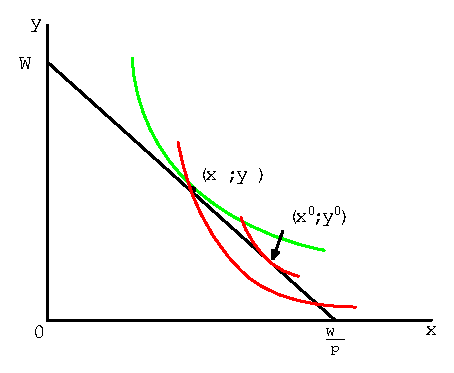
\epsfig{file=best_reply_fig1.eps}}{}

Start with a situation in which Bob's consumption of good $x$ is $x_0$.
Alice's preferences in this case lead her to choose the bundle $( x^{\ast},
y^{\ast} )$ which is the highest indifference curve touching her budget set.
If Bob increases his consumption to $x_0 + d x_0$, then Alice's indifference
curves become steeper, like the red curves in the figure. The tangency then
moves to the right to the point $( x', y' )$. Thats about all there is to it.

The consumer's demand function is a type of best reply function. It is common
to think of the demand function in a graphical way, sloping downwards and
eventually meeting some kind of supply function. We can do the same kind of
thing for any best reply function. Here we don't care so much about changes in
price and income, but we do care about the impact of a change in Bob's
consumption.

The next Figure summarizes what we have figured out.

\tmfloat{h}{small}{figure}{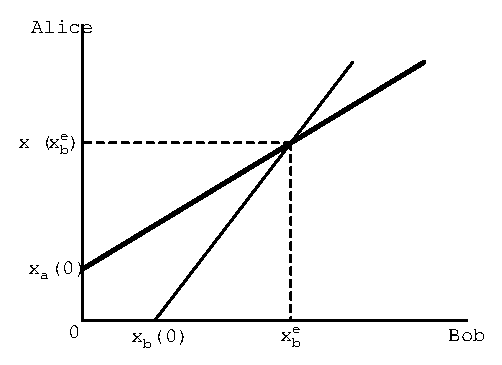
\epsfig{file=best_reply_fig2.eps}}{}

The horizontal axis measure Bob's consumption of good $x$, the vertical axis
measures Alice's consumption of good $x$. The thick upward sloping line
records Alice's best reply to Bob's choice. When Bob chooses not to consume
any $x$ at all, Alice still finds that the highest indifference curve touching
her budget line touches at a point whose $x$ coordinate is $x^{\ast} ( 0 )$.
On the other hand, if Bob chooses the higher consumption $x^e_b$, then Alice
finds that her tangency occurs at a new point given by $x^{\ast} ( x^e_b )$
because her indifference curves have all become steeper.

We could do exactly the same sort of exercise for Bob, assuming that his
preferences are also changed by Alice's consumption. The axis are already
labelled the right way, just think of the curves the other way around. For
instance, if Alice chooses to consume 0 units of good $x$, Bob is still likely
to want some. The amount that he wants is determined by his best reply
function which gives an $x$ value of $x^{\ast}_b ( 0 )$.

With this observation, we can make the choices that Alice and Bob make
consistent with one another. Alice is really guessing what consumption Bob
will choose. Bob is doing the same. If Alice thinks that Bob isn't going to
consume any $x$, her best choice is $x^{\ast}_a ( 0 )$. But Bob never chooses
0 units of good $x$. You can see this by looking at the graph. No matter what
consumption he thinks Alice will pick, he always chooses a positive
consumption of good $x$. So Alice is going to see that she is wrong and start
changing her beliefs about Bob. This in turn will cause here to change her
consumption. It seems pretty compelling that things will settle down when Bob
and Alice's beliefs about each other are correct. This happens when Alice
consumes $x^e_a$ and Bob chooses $x^e_b$ - the point where their best reply
functions meet.

This is a pretty big conceptual leap. We can't really predict what Alice is
going to do in this case without knowing what Bob is going to do. We can't say
anything about Bob without knowing what Alice is going to do. We seem to be at
an impasse. What saves us is the best reply concept. The way to understand
what Alice and Bob do is to think about the things they could have done, but
didn't. In economic history, this idea is called {\tmem{counter factual
analysis}}. Historians love to imagine what the Canadian Economy would look
like if the rail line had never been built to the west coast, or what the
American Economy would look like without the American civil war. We do the
same - what would Alice do in all the counter factual situations that she
might encounter with Bob. Then we can consider each of these counterfactuals
and try to think through whether they make sense.

The point of this section is not so such much to show you how to do this. You will
learn this method when you study game theory. The point here is to show how
our utility theorem is making it possible to do this. Considering all possible
counterfactuals is an impossible task using words and intuition - there is
just too much to think about. The maximization approach suggested by the
utility theorem allows us to reduce these counterfactuals to very simple
geometrical and mathematical objects that we can manipulate.

\subsection{An algebraic Treatment}

An alternative approach to the one described above is to provide enough
structure on the preferences of Alice and Bob that we can find their best
reply functions explicitly. Suppose that Alice's utility function is $u ( x_a,
y_a, x_b ) = x_a^{\alpha ( x_b )} y_a^{1 - \alpha ( x_b )}$ where we are going
to let
\begin{equation}
  \text{$\alpha ( x_b ) \equiv \frac{p x_b}{W} \left( \frac{3}{4} \right) +
  \frac{W - p x_b}{W} \left( \frac{1}{4} \right)$}
\end{equation}
because we need something concrete to find the best reply functions
explicitly.

If you recall, the marginal rate of substitution of $y$ for $x$ is given by
the ratio of the marginal utility of good $x$ to the marginal utility of good
$y$. In words, this is the amount of good $y$ the consumer would be willing to
give up in order to get 1 additional unit of good $x$. The MRS is then given
by
\[ \frac{\alpha ( x_b ) x^{\alpha ( x_b ) - 1} y^{1 - \alpha ( x_b )}}{( 1 -
   \alpha ( x_b ) ) x^{\alpha ( b )} y^{- \alpha ( x_b )}} = \frac{\alpha (
   x_b ) y}{( 1 - \alpha ( x_b ) ) x} \]
This is an increasing function of $x_b$, because $\frac{d \alpha}{d x_b} =
\frac{1}{2} \frac{p}{W} > 0$.

From our previous work, we know that the $x$ coordinate of the bundle that
maximizes Alice's utility is
\begin{equation}
  x^{\ast}_a ( x_b ) = \frac{\alpha ( x_b ) W}{p} = \frac{( W + 2 p x_b )}{4
  W} \frac{W}{p} = \frac{W + 2 p x_b}{4 p} \label{exp}
\end{equation}
Now we can put some more structure on the diagram that is given above. For
example it is immediate from (\ref{exp}) that the intercept of Alice's best
reply function is $x^{\ast}_a ( 0 ) = \frac{W}{4 p}$. This function is linear
and has slope $\frac{1}{2}$.

If Bob has the same preferences, then his best reply function looks exactly
the same. For their choices to be consistent with one another we want both
Alice and Bob to guess each other's actual consumption correctly. In other
words, Alice's guess about what Bob would do, $x_b$ is equal to what Bob
actually does do when he correctly predicts Alice's consumption, $x^{\ast}_a (
x_b )$. That is
\[ x_b = x^{\ast}_b \left[ x^{\ast}_a ( x_b ) \right] \]
Notice how this works. We start with Bob's consumption and use this to find
Alice's consumption. We take the result and use it find Bob's consumption. If
we get the consumption level we started with, then we have found the
consumption levels that are consistent with one another.

Lets try this in the previous diagram.

\tmfloat{h}{small}{figure}{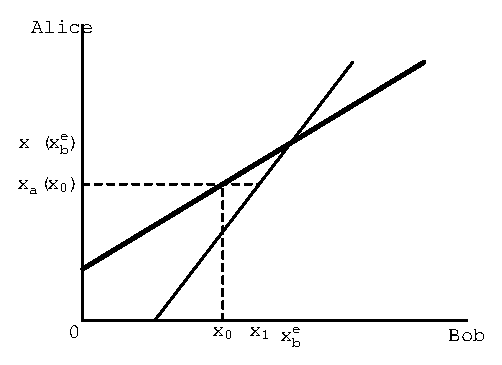
\epsfig{file=best_reply_fig3.eps}}{}

Start with Bob's consumption. In the diagram this is $x_0$ and is labelled on
the horizontal axis, where Bob's consumption is measured. We need to compute
Alice's consumption. From (\ref{exp}), this is
\[ x^{\ast}_a ( x_0 ) = \frac{W + 2 p x_0}{4 p} \]
Using this, we can compute Bob's consumption by measuring the (horizontal)
distance over to his best reply function. This would be
\[ x^{\ast}_b ( \frac{W + 2 p x_0}{4 p} ) = \frac{W + 2 p \left( \frac{W + 2 p
   x_0}{4 p} \right)}{4 p} = x_1 \]
It should be clear from the diagram that this won't give us the right answer
unless we choose $x_0$ at the point where the best reply functions cross. From
the algebra above, this is simply the solution to
\[ \frac{W + 2 p \left( \frac{W + 2 p x}{4 p} \right)}{4 p} = x_{} \]
or
\[ \frac{W}{2} = p x \]
This is a simple Nash equilibrium.

\end{document}
